\documentclass[11pt, a4paper, oneside]{ctexart}
\usepackage{amsmath, amsthm, amssymb, appendix, bm, graphicx, hyperref, mathrsfs, float,subfigure,booktabs,tabularx,longtable,geometry,pdfpages}
%\usepackage{fancyhdr}	%用于更改默认的页眉页脚格式
\usepackage{listings}  % 用于插入代码
\usepackage{xcolor}  % 用于设置颜色
\usepackage{caption}
\usepackage{cite}
\usepackage{multirow}

\captionsetup{font=small}
\renewcommand {\thetable} {\thesection{}.\arabic{table}}
\renewcommand {\thefigure} {\thesection{}.\arabic{figure}}

\title{\heiti\zihao{-1}\textbf{科学研究与创新实践中期报告}}
\date{}


\graphicspath{{img/}}

\begin{document}

\begin{figure}
    \centering
    
\includegraphics[scale=1.2]{SJTU}
\end{figure}
\maketitle

\begin{table}[h]
    \centering
    \begin{tabular}{>{\bfseries\zihao{4}}c@{\zihao{4}\textbf{:}}>{\centering\arraybackslash\zihao{-4}}p{8cm}}
        题目 & 一种藤蔓式软体生长机器人的设计与控制 \\
        \cline{2-2}
        姓名 & 陈乐凯 \\
        \cline{2-2}
        学号 & 521020910180 \\
        \cline{2-2}
        导师 & 谷国迎 \\
        \cline{2-2}
        专业 & 机械工程 \\
        \cline{2-2}
        日期 & 2024.2.19 \\
        \cline{2-2}
    \end{tabular}
\end{table}
\thispagestyle{empty}

\newpage
\setcounter{page}{1}
\pagenumbering{Roman}
\tableofcontents

\newpage
\setcounter{page}{1}
\pagenumbering{arabic}
\section{课题背景与研究现状}
生长作为一种广泛存在于生物(尤其是植物界)发育、繁衍和扩散的机制,依靠尖端生长增加其本身的长度,使得生物体能够不断适应和突破环境,
其优势在于能够使得生物再相对受限的环境中进行自适应运动,尽可能减少环境阻碍的影响,如图\ref{生长过程说明}所示。

\begin{figure}[H]
    \centering
    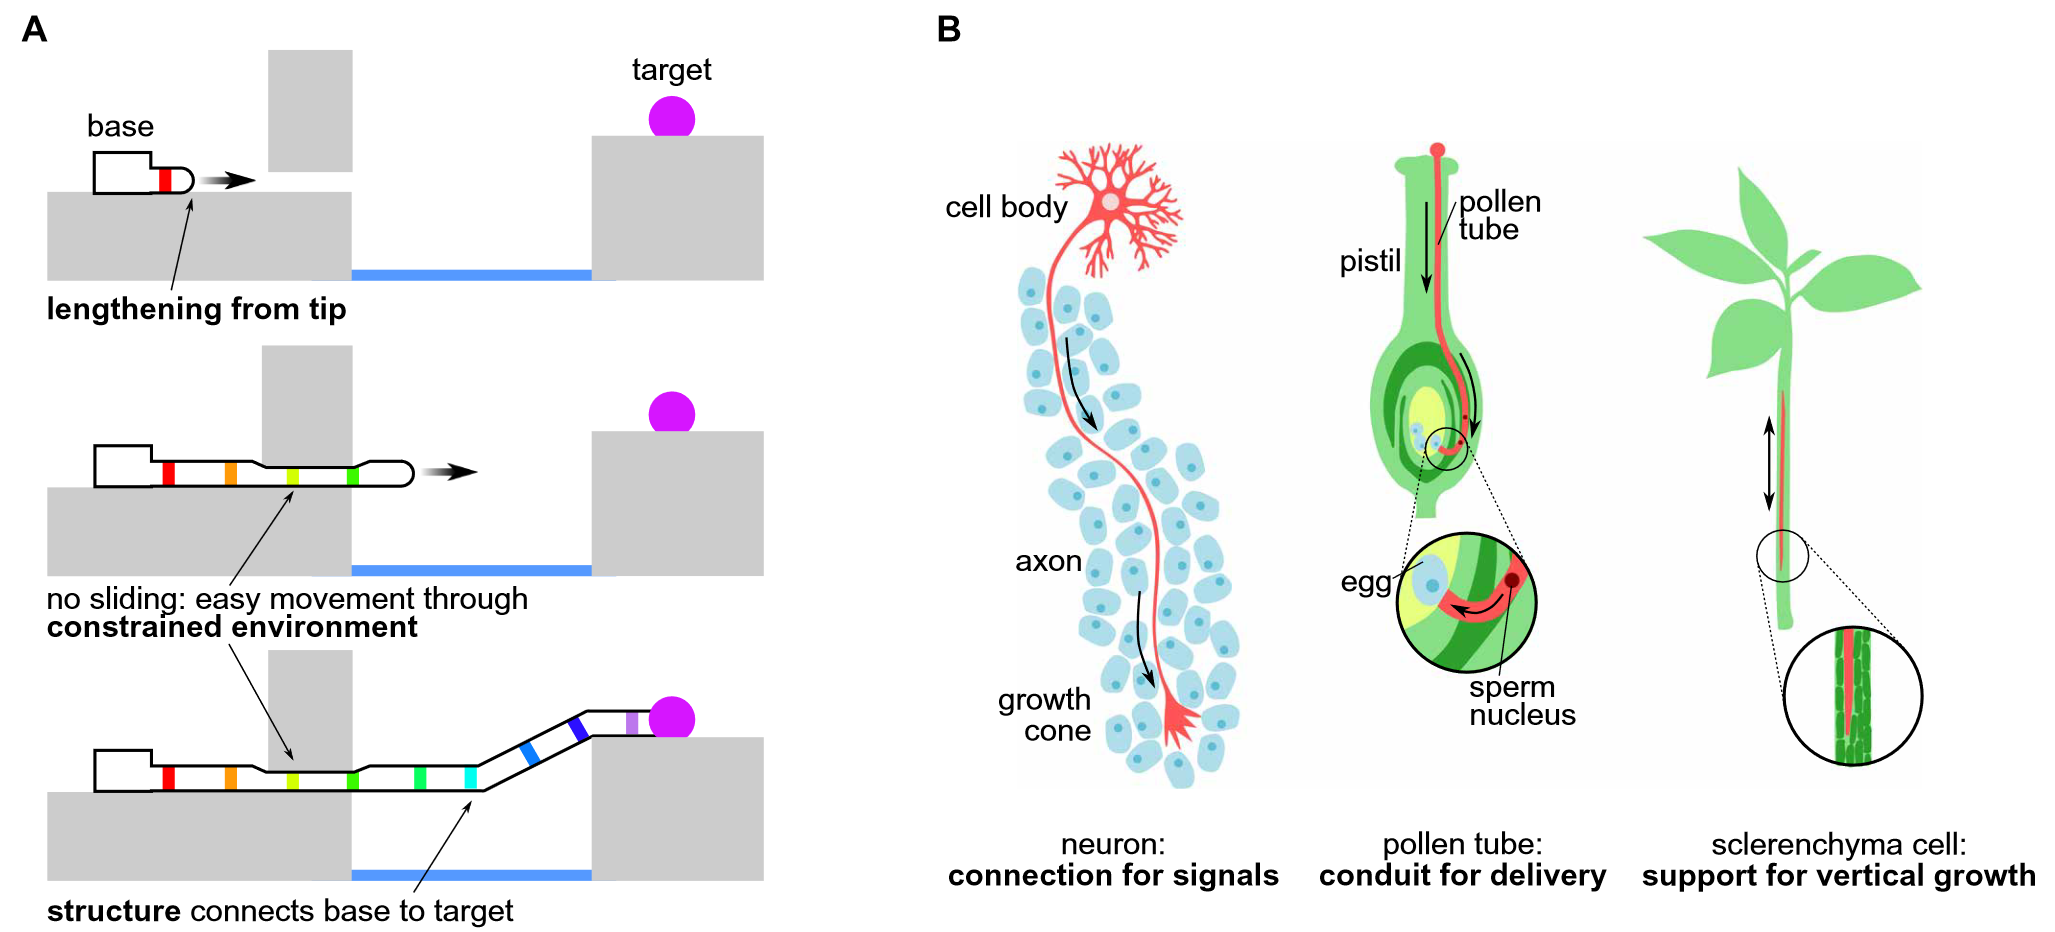
\includegraphics[scale=0.2]{生长过程说明}
    \caption{生物体通过生长通过相对受限的环境\cite{hawkesSoftRobotThat2017a}(A)生长过程说明。生长过程中只有尖端移动,而中段相对环境并不发生相对移动,从而减少了运动阻力(B)生物系统中生长的例子。神经元通过组织间隙生长,花粉管通过雌蕊组织间隙生长,厚壁组织细胞在木质部和韧皮部内生长}
    \label{生长过程说明}
\end{figure}

在世界机器人领域蓬勃发展的今天,具有高灵活度和适应性的软体机器人是备受关注的领域之一,
其在环境勘测、生物医学、人机交互等领域的有着巨大的应用前景,其中,
一种类似藤蔓运动模式,依靠气动生长的机器人因其独特优势备受关注:

(1)通过气动反转材料,可以在不接触环境的情况下进行运动;

(2)气动的驱动模式在给予了该机器人足够刚度的同时又有一定的柔性,使得其能够适应各种复杂的工作环境,例如狭缝、流体等;

(3)由于机器人主体的薄膜材料本身的质量体积较小,使得其不仅便于收纳,又有很大的扩展延伸的潜力,在Hawkes等人的研究中\cite{hawkesSoftRobotThat2017a},这种生长机器人的最大长度能够达72米,最大生长速度达10米每秒,远远超过当前有类似功能的绳牵引机器人或尺蠖机器人;

(4)由于软体的特性,机器人对环境的破环较小\cite{coadRetractionSoftGrowing2020},具有在复杂环境勘测和生物医学检查领域应用的潜质;

(5)目前翻转式生长机器人的主体部分一般由聚丙烯塑料制成,成本和制造难度相对于一般刚性机器人低,结构较为简单,鲁棒性高。

\section{工作机理与实物设计}

\subsection{整机工作机理}
Hawkes等人在论文中\cite{hawkesSoftRobotThat2017a},通过无脊椎动物内陷附肢的运动机理,设计了一种基于薄膜在内压驱动下的外翻
生长机构,并通过聚乙烯薄膜实现了该机构,通过实验发现,这种机构在生长速度、生长长度和运动控制方面具有显著的优势和拓展潜力,因此
本文参考上述机构,并针对长度控制和压力控制进行一定改进,使得机器人能够有更强的鲁棒性和更好的控制性,具体工作机理如图\ref{工作示意图}所示。

\begin{figure}[H]
    \centering
    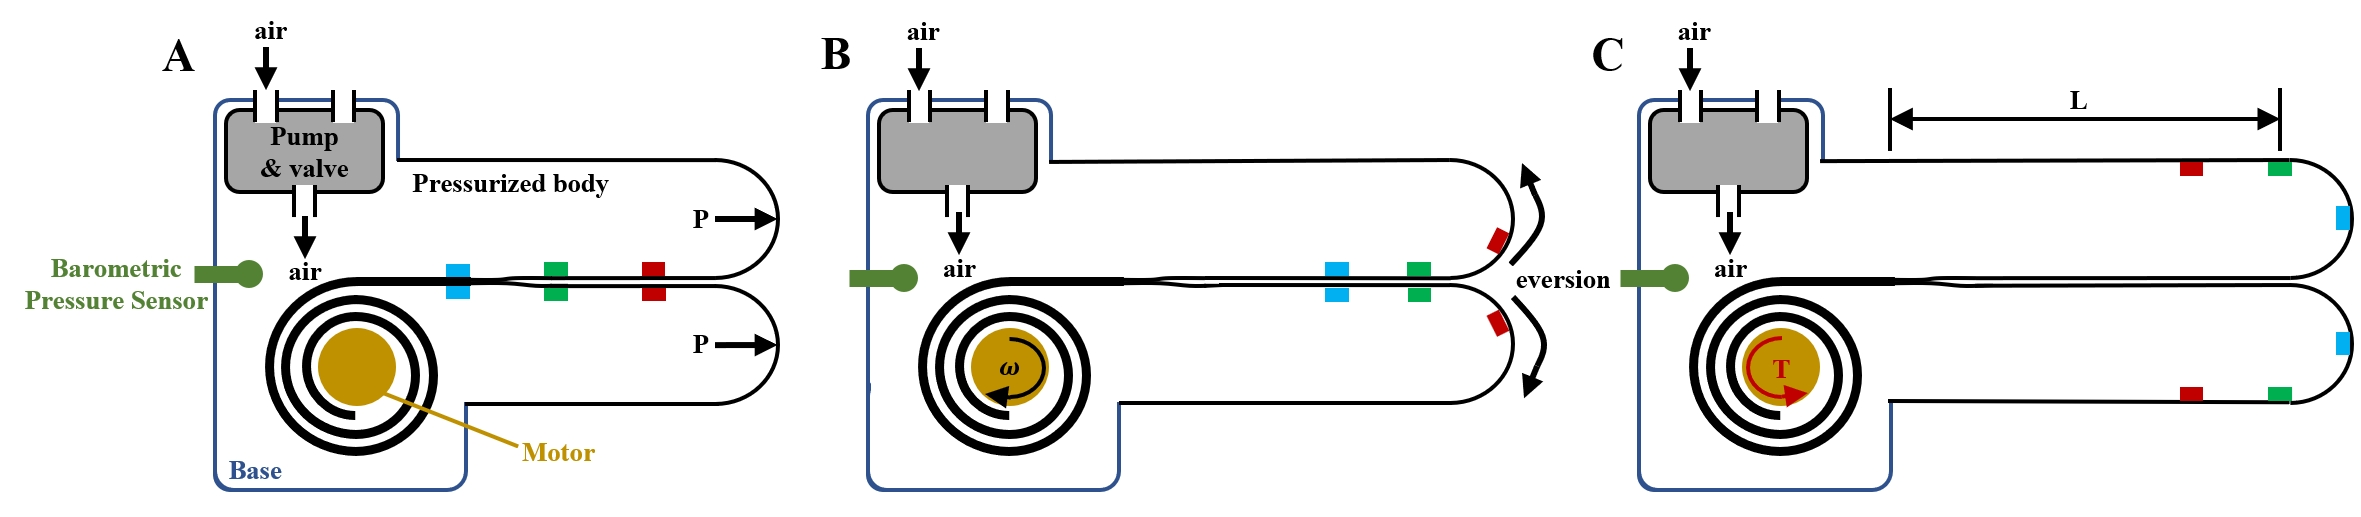
\includegraphics[scale=0.18]{工作示意图}
    \caption{基于Hawkes等人研究的改进模型(A)气泵充气创造一个压力相对较大的内腔(B)由于压力差,薄膜实现自主外翻(C)通过电机施加扭矩控制生长长度}
    \label{工作示意图}
\end{figure}

改进的模型主要由基座、充气主体,泵阀管路以及压力传感器构成(如图\ref{工作示意图}A所示),首先通过充气创造一个压力相对较大的内腔,使得机器人主体有一定的刚度,同时,
考虑到基座和主体连接的气密性并不一定完全理想,因此压力传感器实时监测内腔压力,并驱动气泵运行控制内腔压力保持相对恒定。当电机轴旋转时,被卷收的塑料薄膜被释放,在内部压力的
作用下,主体内层材料向外翻折,使得主题长度伸长,达到生长的效果(如图\ref{工作示意图}B所示)。根据电机轴旋转角度和主体伸长长度的关系,通过旋转一定角度使得主体伸长到目标长度后,
电机轴停转并提供反向扭矩平衡由于内外压力差对电机轴产生的扭矩,实现生长长度控制。

\subsection{生长长度计算}
由上述机理可知,机器人通过控制电机旋转圈数控制生长长度,为了准确定量描述和控制生长长度,可以将卷收抽象为如下问题。

\begin{figure}[H]
    \centering
    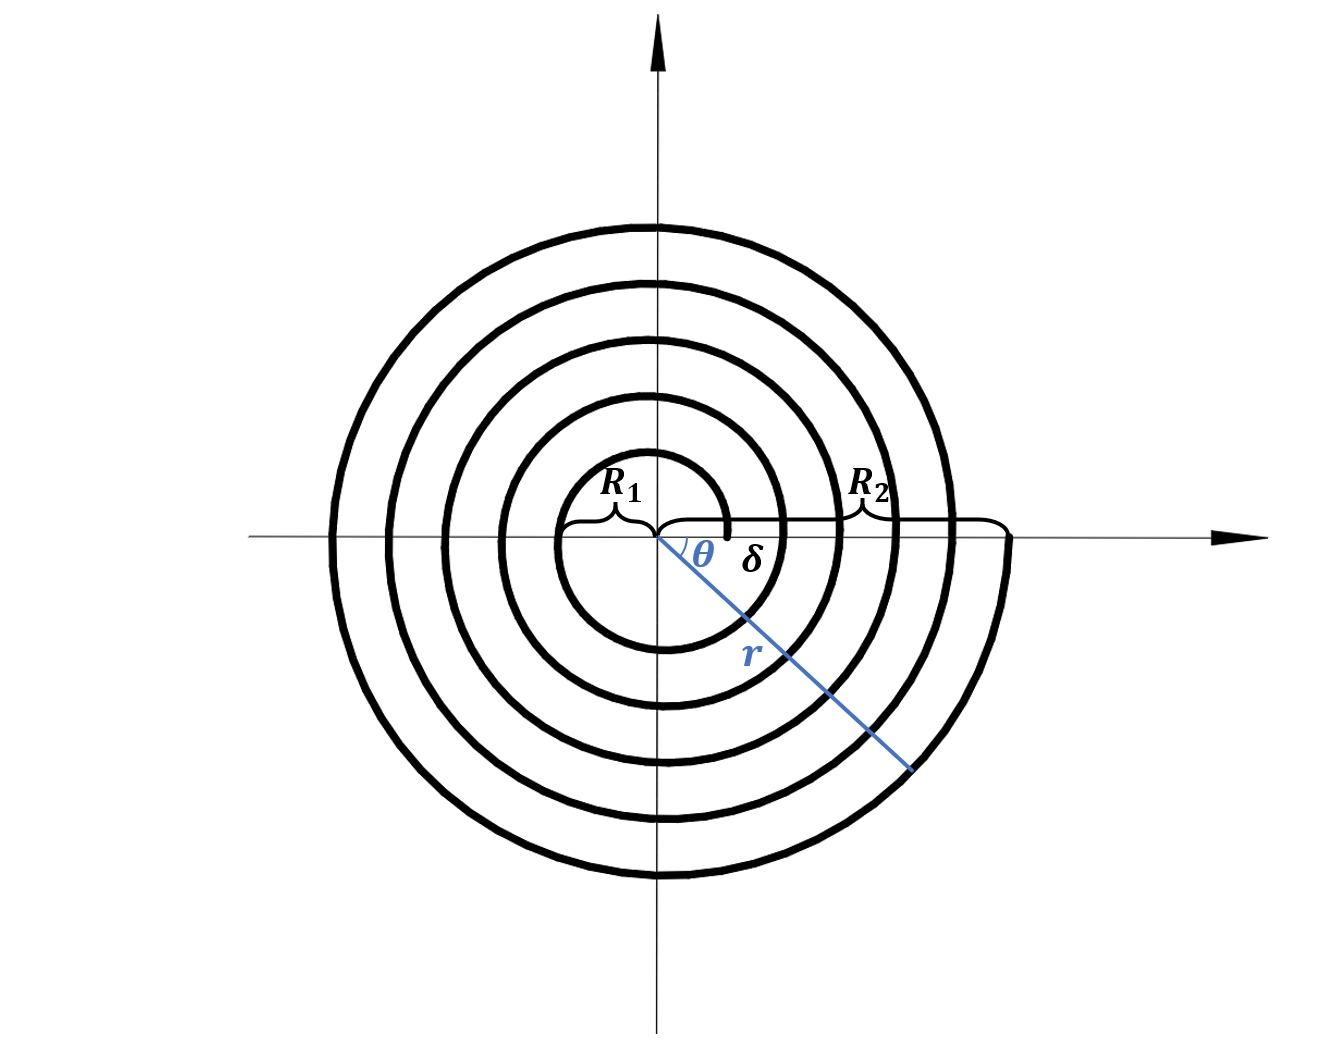
\includegraphics[scale=0.2]{阿基米德曲线积分}
    \caption{阿基米德曲线积分}
    \label{阿基米德曲线积分}
\end{figure}

当电机轴旋转一周时,卷收薄膜的半径的变化量为一个薄膜的厚度,并且可以认为在各处卷收薄膜的半径随旋转角度的变化率$\frac{dr}{d\theta}$相同,因此如果将薄膜中线单独考虑即为一个阿基米德曲线,如图\ref{阿基米德曲线积分}
所示,设滚筒(由电机轴控制)半径为$R_1$,薄膜圈数为$n$,单层薄膜厚度为$\delta$,则
$$
R_2=R_1+n\delta
$$
设旋转角度为$\delta$,卷收薄膜的半径随弧度的变化率为$\frac{dr}{d\theta}=\frac{\delta}{2\pi}$则
$$
r=R_2-\theta \frac{dr}{d\theta}=R_1+n\delta-\theta \frac{\delta}{2\pi}
$$
根据极坐标下的曲线公式
$$
L=\int_{\theta_1}^{\theta_2}\sqrt{r^2+\left(\frac{dr}{d\theta}\right)^2}d\theta
$$
由于此时变化率$\frac{dr}{d\theta}=\frac{\delta}{2\pi}$远小于半径$r$,因此可以忽略积分中的变化率项,得到长度与旋转角度
近似关系为
$$
L=(\theta_2-\theta_1)[(R_1+n\delta)-(\theta_2+\theta_1)\frac{\delta}{4\pi}]
$$
可以看到,当旋转角度较小时,生长长度正比于旋转角度。
$$
L\approx \Delta\theta(R_1+n\delta)\propto \Delta\theta
$$

\subsection{实物设计模型}
根据上述机理模型,设计实物模型如图\ref{模型草图}所示。

\begin{figure}[H]
    \centering
    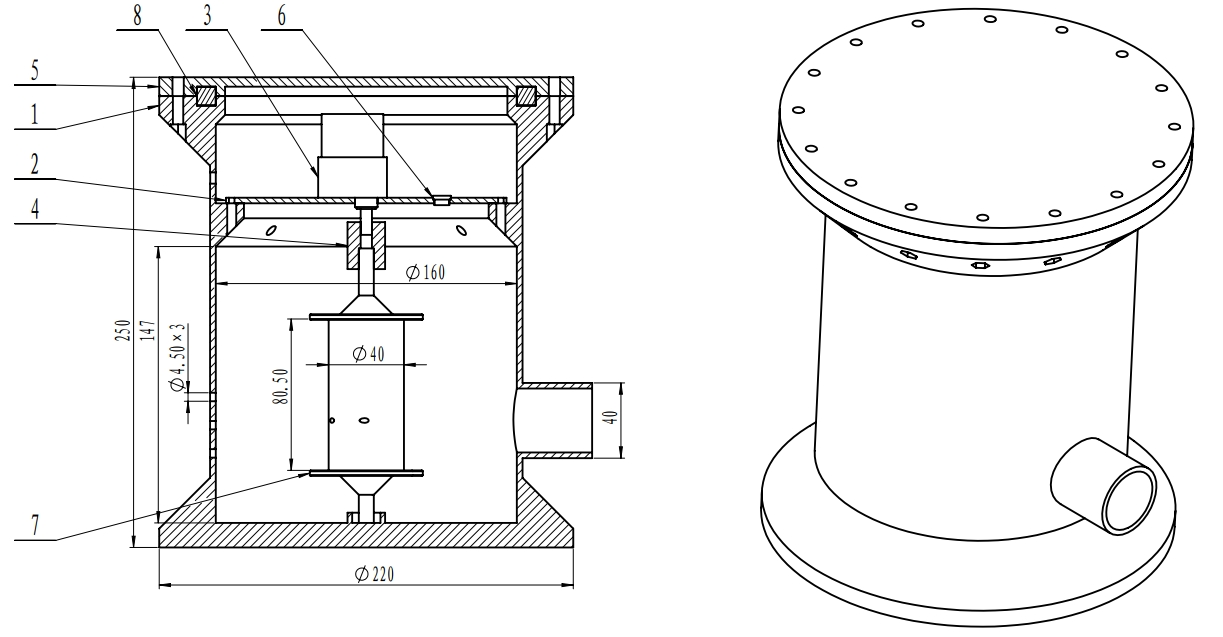
\includegraphics[scale=0.3]{模型草图}
    \caption{模型及其内部结构示意图(1.基座2.基座盖3.直流电机4.联轴器5.基座盖6.摄像头7.滚轴8.硅胶密封圈)}
    \label{模型草图}
\end{figure}

为了保证整体的密封性,模型整体都被包含在基座和基座盖构成的密封空间中(即上文中的加压内腔),其中直流电机(3)和
滚筒(7)由联轴器(4)进行连接,滚筒上设计有通孔和平台,分别用于固定和防止塑料薄膜,而机体上设计有圆柱形开口,
作为塑料薄膜(机器人生长)的出口,此外,在基座内部贴放了LED灯带和摄像头(6),便于观察基体的内部情况和塑料薄膜的形态。

\begin{table}[H]
    \centering
    \caption{实物部分尺寸表}
    \label{实物部分尺寸表}
    \begin{tabular}{cc}
        \toprule
        结构名称 & 具体尺寸(mm) \\
        \midrule
        基体外径 & 220.0 \\
        基体总高 & 250.0 \\
        基体内径 & 160.0 \\
        滚筒有效高度 & 80.5 \\
        滚筒直径 & 40.0 \\
        管路、电路孔径 & 4.5 $\times$ 3 \\
        薄膜出口外径 & 40 \\
        \bottomrule
    \end{tabular}    
\end{table}

\begin{figure}[H]
    \centering
    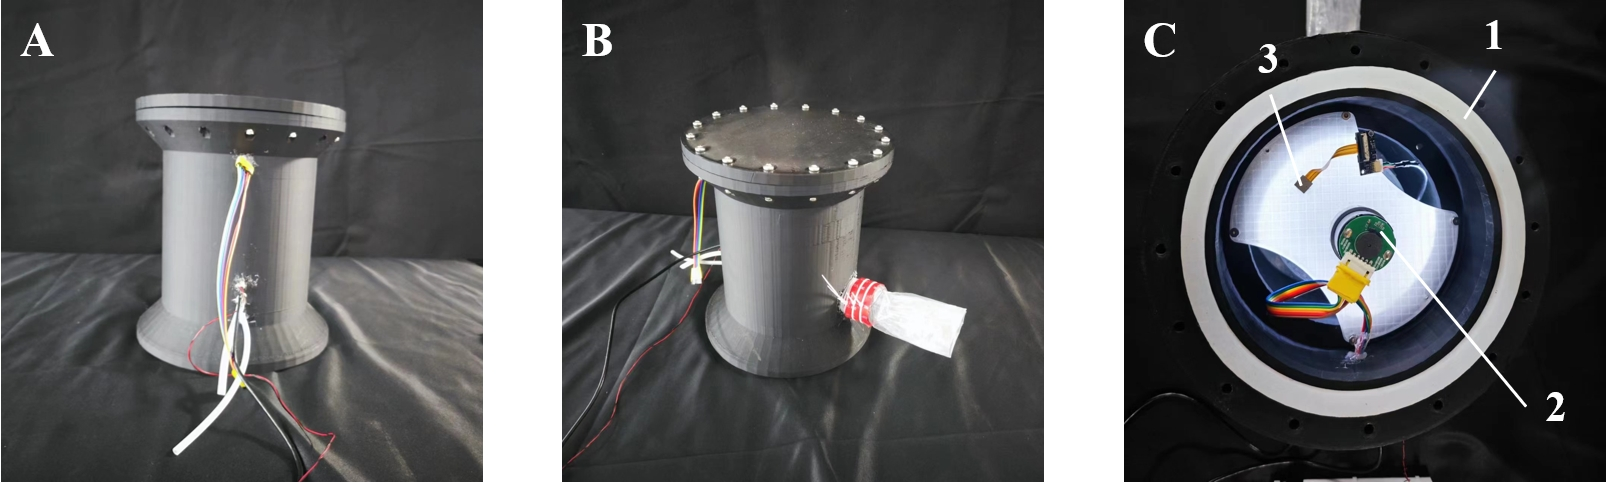
\includegraphics[scale=0.25]{外部图}
    \caption{实物图(A)电机线与气路管道(B)实物轴测图(C)内部图(1.硅胶密封圈2.直流电机3.摄像机)}
    \label{外部图}
    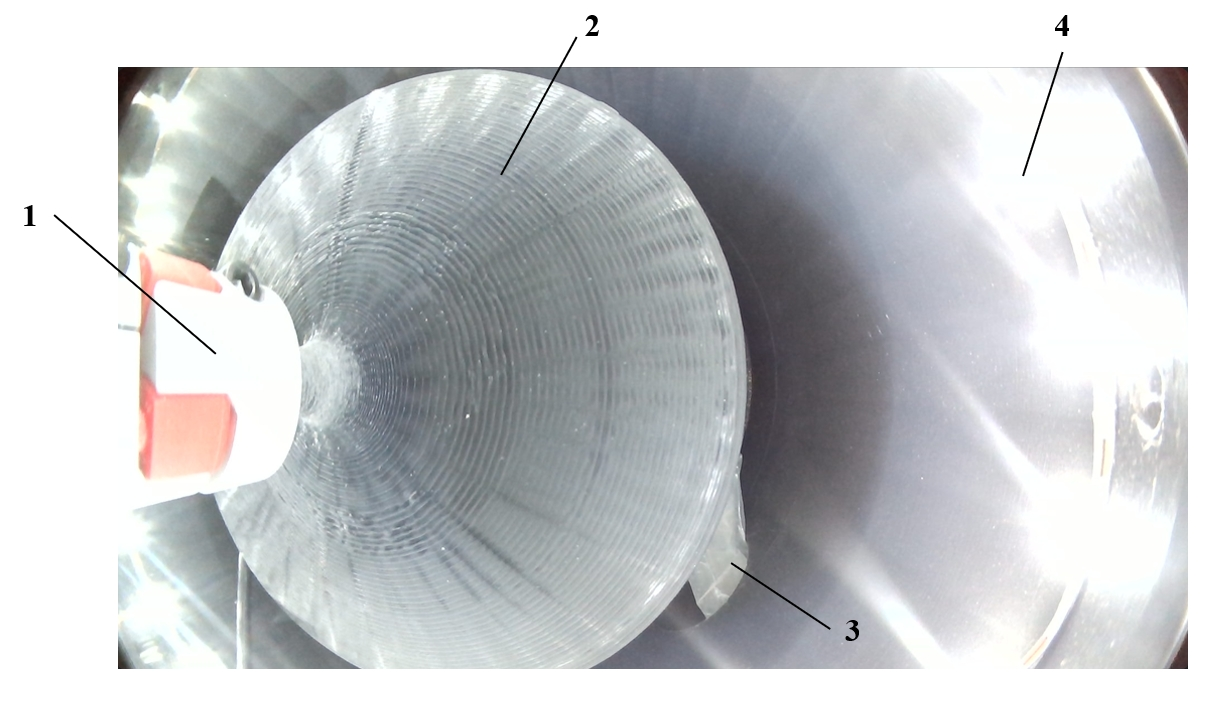
\includegraphics[scale=0.3]{内部图}
    \caption{内部摄像机画面(1.联轴器2.滚筒3.塑料薄膜4.LED灯带}
    \label{内部图}
    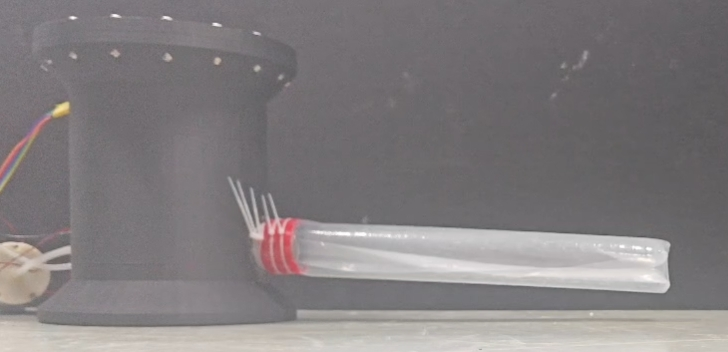
\includegraphics[scale=0.5]{生长图}
    \caption{机器人工作状态(充气)图}
    \label{生长图}
\end{figure}

\section{控制与算法设计}
\begin{figure}[H]
    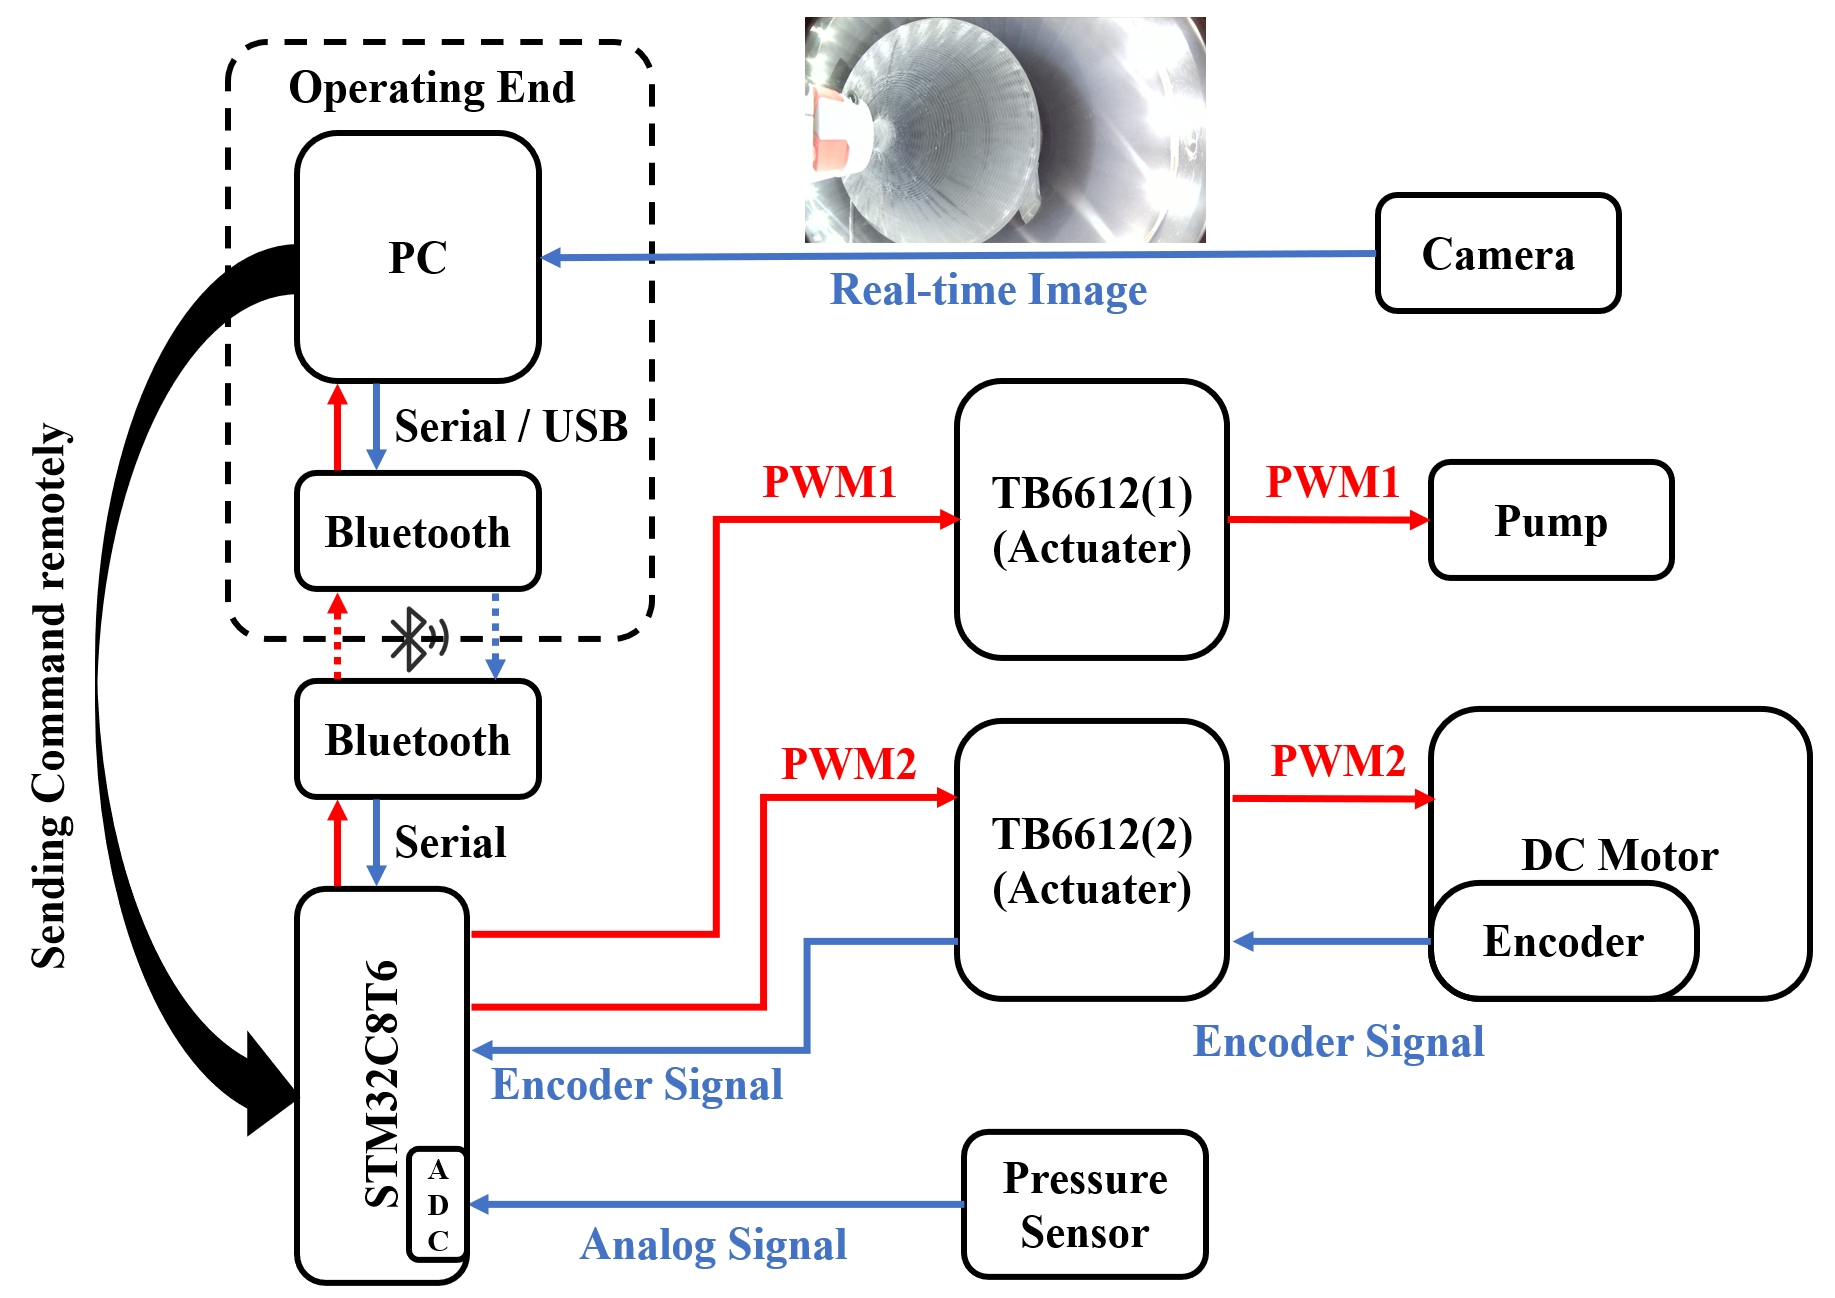
\includegraphics[scale=0.2]{器件连接原理图}
    \caption{器件连接原理图}
    \label{器件连接原理图}
\end{figure}

基于机理图\ref{工作示意图},设计器件连接原理图如图\ref{器件连接原理图}所示,
通过STM32C8T6单片机对泵、直流电机和传感器进行控制或者数据采集,其中泵本质上
也是直流电机,因此都利用TM6612芯片作为驱动器对其进行控制;直流电机带有霍尔
编码器(增量式编码器),单片机通过解析编码器方波信号,能够获取电机的转速、
位置等信息;压力传感器(40PC100G2A)能够输出0-4V的模拟信号,通过单片机ADC外设
转换即可由对应的电压信号获得内腔压力数值。

同时,为了便于观测基座内部情况以及调试和控制机器人生长,额外设计了PC操作端,通过
蓝牙通信远程发送机器人指令(控制内腔气压、生长长度),简化了操作流程,此外,
通过摄像机捕捉内腔的实时图像并传输回PC,也能够监测内腔中塑料薄膜的状态、位置信息。

根据上述生长机理,指定机器人生长控制逻辑图如下。
\begin{figure}[H]
    \centering
    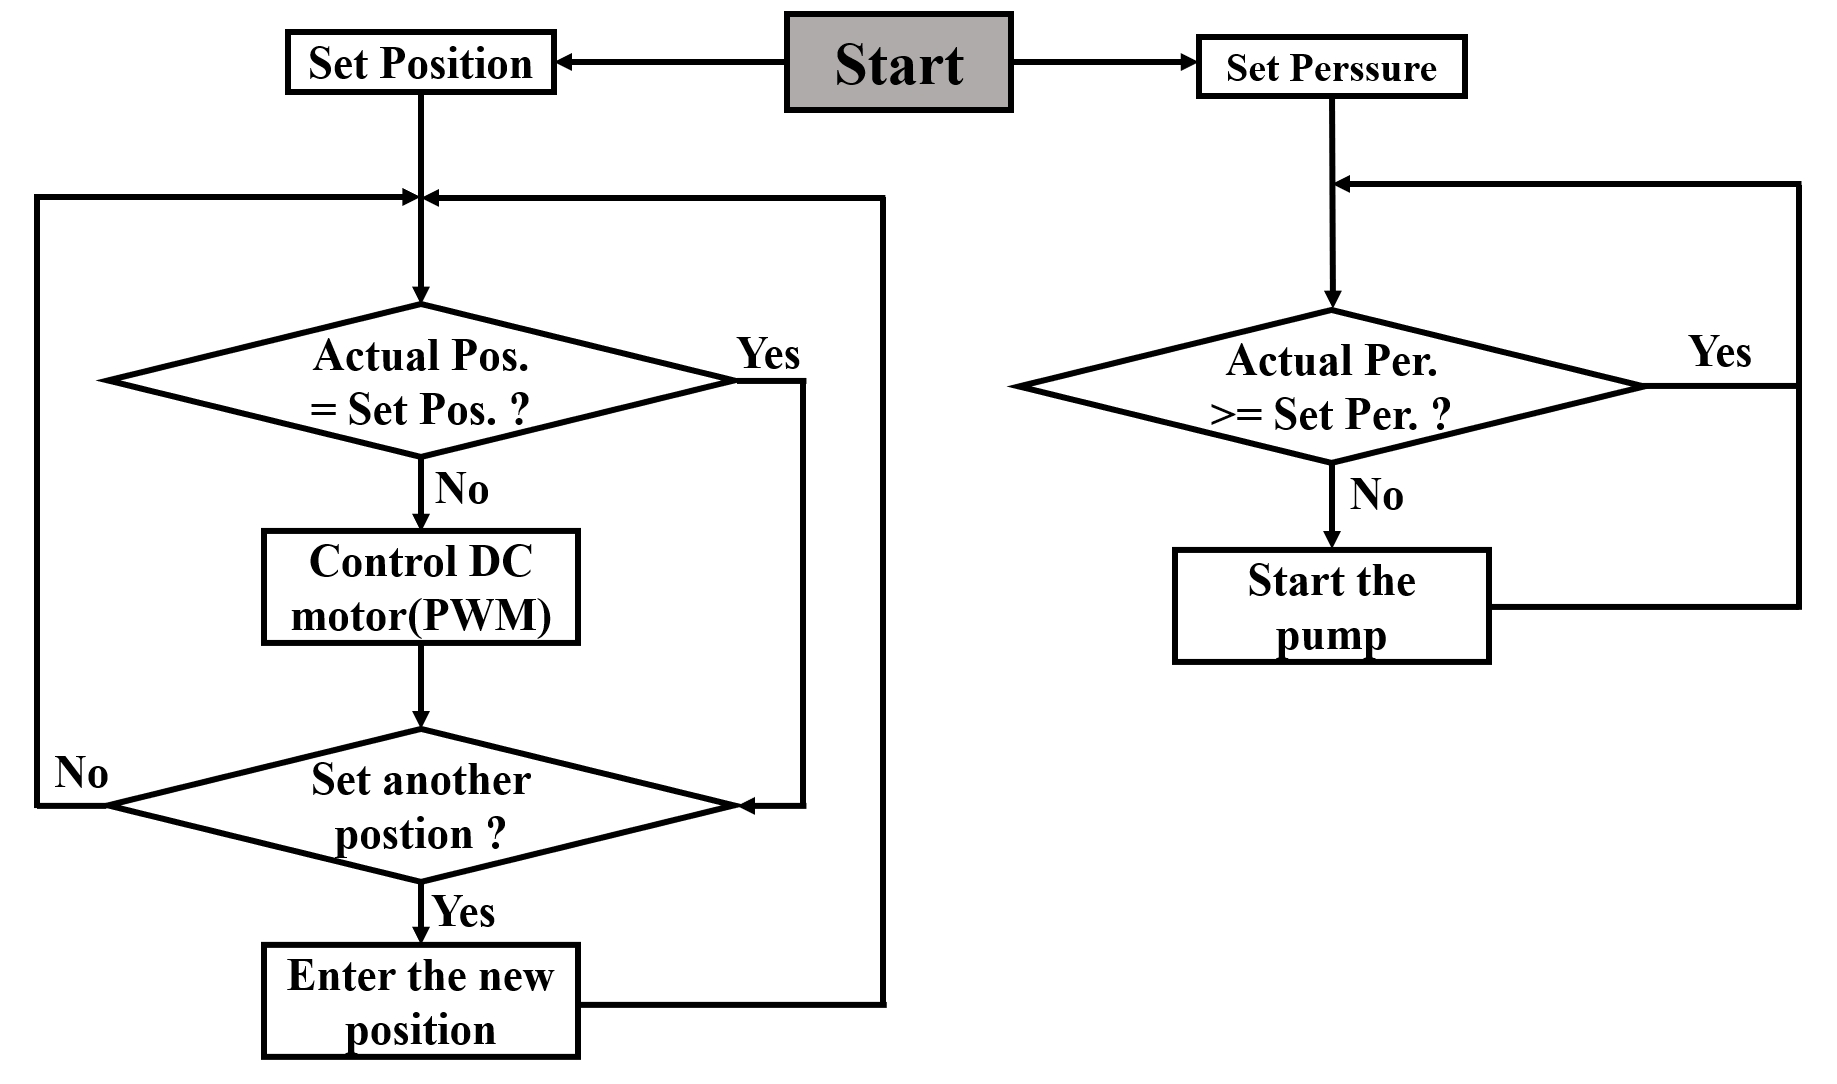
\includegraphics[scale=0.2]{控制框图}
    \caption{机器人生长控制逻辑图}
    \label{控制逻辑图}
\end{figure}

可以看到,气泵-压力传感器用于保持内腔的气压恒定,而直流电机-编码器用于控制机器人生长长度,
二者相互解耦,对于控制上能够很大程度地简化流程。

下面的部分将分别介绍各个外部设备的调试过程和控制方案(气泵同样相当于直流电机,
并且仅采用阈值控制弥补气密性缺陷,无需对其位置,速度进行控制,这里省略气泵的控制方案)。

\subsection{电机检测与控制}
为了使机器人能够生长特定的长度,则需要控制电机轴转动对应的角度(详见2.2节计算),为了保证电机的角度(位置)要准确可靠,
需要知道当前电机的位置并与设定值比较后进行闭环控制,实验中利用编码器进行位置测量,并结合电机PID控制,实现了较为准确的角度控制。
\subsubsection{编码器调试与测量}
\begin{figure}[H]
    \centering
    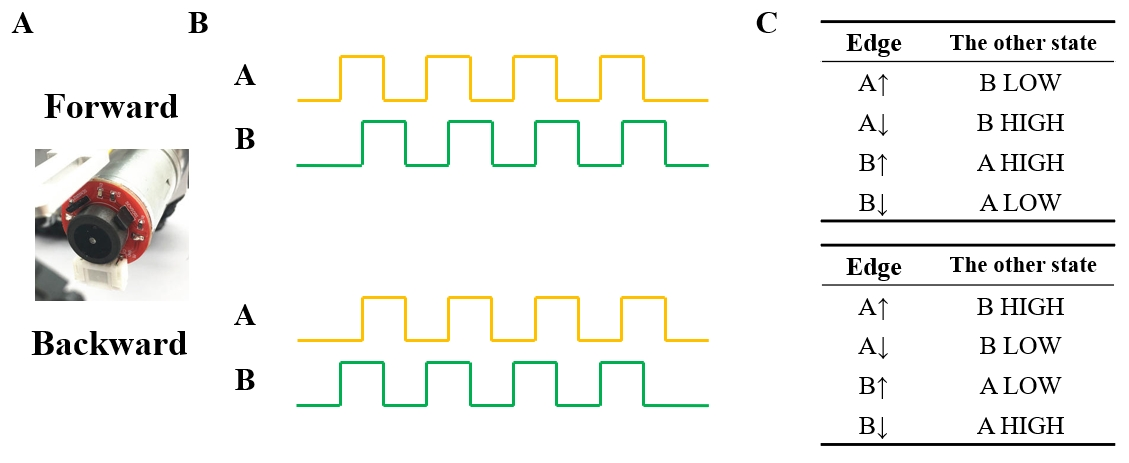
\includegraphics[scale=0.38]{编码器电平图}
    \caption{霍尔编码器检测原理(A)霍尔编码器在直流电机上的安装,两个霍尔元件安装位置差90度,能够产生相位差90度的方波信号(B)电机正转和反转时两相信号的特征(C)通过检测边沿信号进行计数,从而反应电机轴位置,并通过另一相信号的高低电平情况能够判断电机转向}
    \label{编码器电平图}
\end{figure}

霍尔增量式编码器检测原理与信号方波图如图\ref{编码器电平图}所示,当A,B其中一相出现上升沿或者下降沿时,进行一次计数,显然,一个方波周期内计数值为4,若编码器线数为$l$(实验中为$13ppr$),电机
减速比为$n$(实验中为$30$),则电机旋转一周的计数值$N$为
$$
N=l\times n \times 4=1560
$$
通过总计数值,即可获得当前电机旋转圈数(位置,角度),此外,通过测量方波频率,或者统计一定时间内的计数值,即可换算电机的转速。
在实验中,采用STM32C8T6单片机定时器外设中寄存器为16位,因此最大计数值位65535,当转动圈数过大或者反向转动时,会发生数据溢出同时
定时器重置,并申请中断,因此在中断函数中需要记录溢出情况,并在计算位置时考虑溢出的次数,算法伪代码如下。

\begin{verbatim}
    // Interrupt function
    function HandlerOfTIM:
        if Counter < 32768:
            OverFlowCounter ++
        else:
            OverFlowCounter --
    
    // Get the current position(Angle)
    function GetPosition:
        return (OverFlowCounter * 65536 + Counter) / 1560.0 * 360
\end{verbatim}

\subsubsection{电机PID控制算法}
获取电机实际位置后,通过与设定位置进行比较,即可对位置进行PID控制,控制框图如下。
\begin{figure}[H]
    \centering
    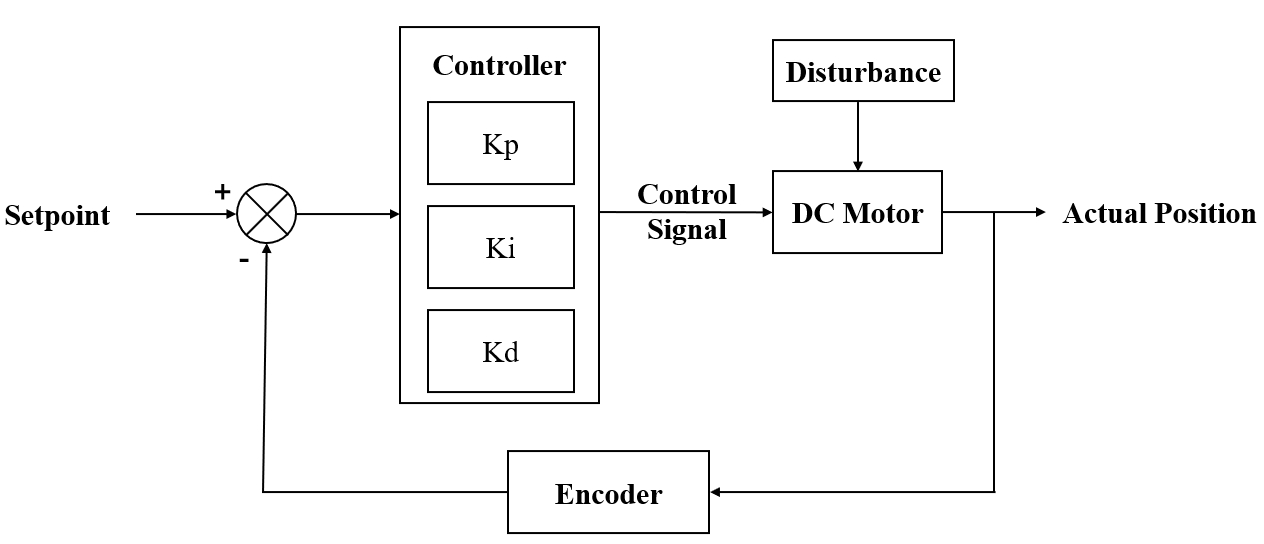
\includegraphics[scale=0.32]{PID}
    \caption{PID控制框图}
    \label{PID}
\end{figure}
由于单片机只能处理离散时间信号,因此由误差值得到的控制信号也应该是离散的,对PID算法进行离散化处理得到
离散时间信号下对应的控制信号计算公式。
$$
u(k)=K_{p}\cdot e(k)+K_i\cdot\sum_{i=0}e(i)+K_{d}\cdot[e(k)-e(k-1)]
$$

控制信号的正负表示控制电机的正反转,而控制信号的大小换算为PWM波的占空比大小,单片机每间隔一定时间采集电机的位置并进行计算,
即可实现电机的位置控制,伪代码如下。
\begin{verbatim}
    // Infinite loop
    Delay(dt)
    Error = Setpoint - Actual position
    Integral = Integral + Error * dt
    Output = Kp * Error + Ki * Integral + Kd * (Error - Last Error)
    Last Error = Error
\end{verbatim}

根据PID三个参数对于系统的不同影响,对系统进行调参,其中$K_p$可以调节速度加快,并且可以减小稳态误差(单纯的比例控制很难完全消除误差),但
比例系数过大会使超调量增大,调节时间加长,动态性能变坏,甚至会使闭环系统不稳定;$K_i$能够提高系统类型,消除稳态误差,提高控制精度(同样存在稳定性问题),
而$k_d$可以使超调量减小,改善系统在调节过程中的动态特性,但微分控制的缺点是对干扰噪声敏感,使系统抑制干扰的能力降低。

最后,根据实验结果,采取的PID参数为
$$
K_p = 1.5,K_i = 0.5,K_d = 0
$$
\subsection{压力传感器调试与测量}
\subsubsection{压力传感器标定}
\begin{table}[H]
    \centering
    \caption{40PC100G2A压力传感器参数}
      \begin{tabular}{ccccc}
      \toprule
      Pressure Range & Null(VDC) & Span(VDC) & Sensitivity,Typ. & Linearity,B.F.S.L.(\%) \\
      \midrule
      \multirow{5}[2]{*}{0 to 100 psi} & \multirow{5}[2]{*}{0.50 ± 0.04} & \multirow{5}[2]{*}{\textcolor[rgb]{ .141,  .125,  .129}{4.00 ± 0.09}} & \multirow{5}[2]{*}{\textcolor[rgb]{ .141,  .125,  .129}{40.0 mV/psi}} & \multirow{5}[2]{*}{\textcolor[rgb]{ .141,  .125,  .129}{0.1}} \\
            &       &       &       &  \\
            &       &       &       &  \\
            &       &       &       &  \\
            &       &       &       &  \\
      \bottomrule
      \end{tabular}%
      \\
      \begin{tabular}{cccc}
        \toprule
              & Null Shift(\%) & Span Shift(\%) & Combined Null and Span Shift(\%) \\
        \midrule
        \textcolor[rgb]{ .141,  .125,  .129}{+25° to -18°C} & \textcolor[rgb]{ .141,  .125,  .129}{±1.25} & \textcolor[rgb]{ .141,  .125,  .129}{±0.75} & \textcolor[rgb]{ .141,  .125,  .129}{±1.50} \\
        \midrule
        \textcolor[rgb]{ .141,  .125,  .129}{+25° to +63°C} & \textcolor[rgb]{ .141,  .125,  .129}{±1.25} & \textcolor[rgb]{ .141,  .125,  .129}{±0.75} & \textcolor[rgb]{ .141,  .125,  .129}{±1.50} \\
        \midrule
        \textcolor[rgb]{ .141,  .125,  .129}{+25° to -45°C} & \textcolor[rgb]{ .141,  .125,  .129}{±2.00} & \textcolor[rgb]{ .141,  .125,  .129}{±1.00} & \textcolor[rgb]{ .141,  .125,  .129}{±2.50} \\
        \midrule
        \textcolor[rgb]{ .141,  .125,  .129}{+25° to +85°C} & \textcolor[rgb]{ .141,  .125,  .129}{±2.00} & \textcolor[rgb]{ .141,  .125,  .129}{±1.00} & \textcolor[rgb]{ .141,  .125,  .129}{±2.50} \\
        \midrule
        \textcolor[rgb]{ .141,  .125,  .129}{+25° to +125°C} & \textcolor[rgb]{ .141,  .125,  .129}{±3.00} & \textcolor[rgb]{ .141,  .125,  .129}{±2.00} & \textcolor[rgb]{ .141,  .125,  .129}{±3.00} \\
        \bottomrule
        \end{tabular}%    
    \label{tab:addlabel}%
  \end{table}%
实验中采用的40PC100G2A压力传感器相关参数如图所示,可以看到传感器输出为0-4V的模拟电压,对应0-100psi的压力数据,其灵敏度为40.0mV/psi,因此需要用到单片机的ADC外设将模拟电压进行量化处理,再换算为对应的压力数值,
而STM32C8T6ADC外设的寄存器大小为12位(对应0-4095的量化值),其满量程电压为3.3V,因此换算流程为:读取寄存器量化值-换算为电压大小-根据灵敏度换算压力大小-单位转换为kPa。

注意到传感器存在零点漂移,因此考虑在传感器上电后先等待电压数值稳定,记录偏移值,再在后续的测量中进行补偿,综上所述,从寄存器量化值到压力的换算公式如下。
$$
Pressure = ((PressValue - ZeroShift) / 4095 * 3.3 * 1000 / 40 * 6.894757)
$$
\subsubsection{原始数据处理(Kalman滤波)}
实验中观察到传感器得到的压力数据有较大的波动,因此需要考虑采用滤波的方法得到相对稳定的数据,这里采用一维的Kalman滤波算法,具体过程如下。

假设时$1,2,...,k$时刻分别对压力$z$测量一个值,得到一系列测量数据$z_1,z_2,...,z_k$,则对x的估计值
$$
\begin{aligned}
    \hat{x}_{k}& =\frac{1}{k}(z_{1}+z_{2}+\cdots+z_{k})  \\
    &=\frac{1}{k}(z_{1}+z_{2}+\cdots+z_{k-1})+\frac{1}{k}z_{k} \\
    &=\frac{1}{k}\cdot\frac{k-1}{k-1}(z_{1}+\cdots+z_{k-1})+\frac{1}{k}z_{k} \\
    &=\frac{k-1}{k}\hat x_{k-1}+\frac{1}{k}\cdot z_{k} \\
    &=\hat{x}_{k-1}-\frac{1}{k}(\hat{x}_{k-1}-z_{k})
\end{aligned}
$$
其中令$\frac{1}{k}=K_g$,成为Kalman增益/因数,改写为
$$
\hat x_k=\hat x_{k-1} + K_g(z_k - \hat x_{k-1})
$$
上述公式可以理解为:当前的估计值=上一次的估计值+系数 $\times$(当前的测量值-上一次的估计值),
当前的估计值与上一次的估计值和这次的测量值有关,是数据综合的结果,可以利用递归进行解算。

在压力传感器测量过程中会产生测量误差$e_{MEA}$,而估计值中又会包含估计误差$e_{EST}$,
定义Kalman增益
$$
K_g=\frac{e_{EST_{k-1}}}{e_{EST_{k-1}}+e_{MEA_k}}
$$
当$e_{EST_{k-1}}\gg e_{MEA_k}$时,上次的估计误差$\gg$这次的测量误差,
此时$K_g\to 1$,此时$\hat x_k=\hat x_{k-1} + 1(z_k - \hat x_{k-1})$
$$
\hat x_k=z_k
$$
即k-1次的估计误差远大于k次的测量误差时,$\hat x_k$趋于第k次的测量值,更信任测量值。

反之当$e_{EST_{k-1}}\ll e_{MEA_k}$时,上次的估计误差$\ll$这次的测量误差,
此时$K_g\to 0$,此时$\hat x_k=\hat x_{k-1} + 0(z_k - \hat x_{k-1})$
$$
\hat x_k=\hat x_{k-1}
$$
即k-1次的估计误差远小于k次的测量误差时,$\hat x_k$趋于第k-1次的估计值,更信任估计值。

因此Kalman滤波伪代码如下:
\begin{verbatim}
    function KalmanFilter:
        Kg=(Error of estimation)/(Error of estimation + Error of measurement)
        Current Output = Last Output + Kg * (Measurement - Last Output)

        Last Output = Current Output
        // update the error of estimation
        Error of estimation = (1-Kg) * Error of estimation
\end{verbatim}

在为了测试Kalman滤波的有效性,在计算机上随机模拟产生一组带噪声的数据,利用Kalman滤波算法,得到的结果如下。
\begin{figure}[H]
    \centering
    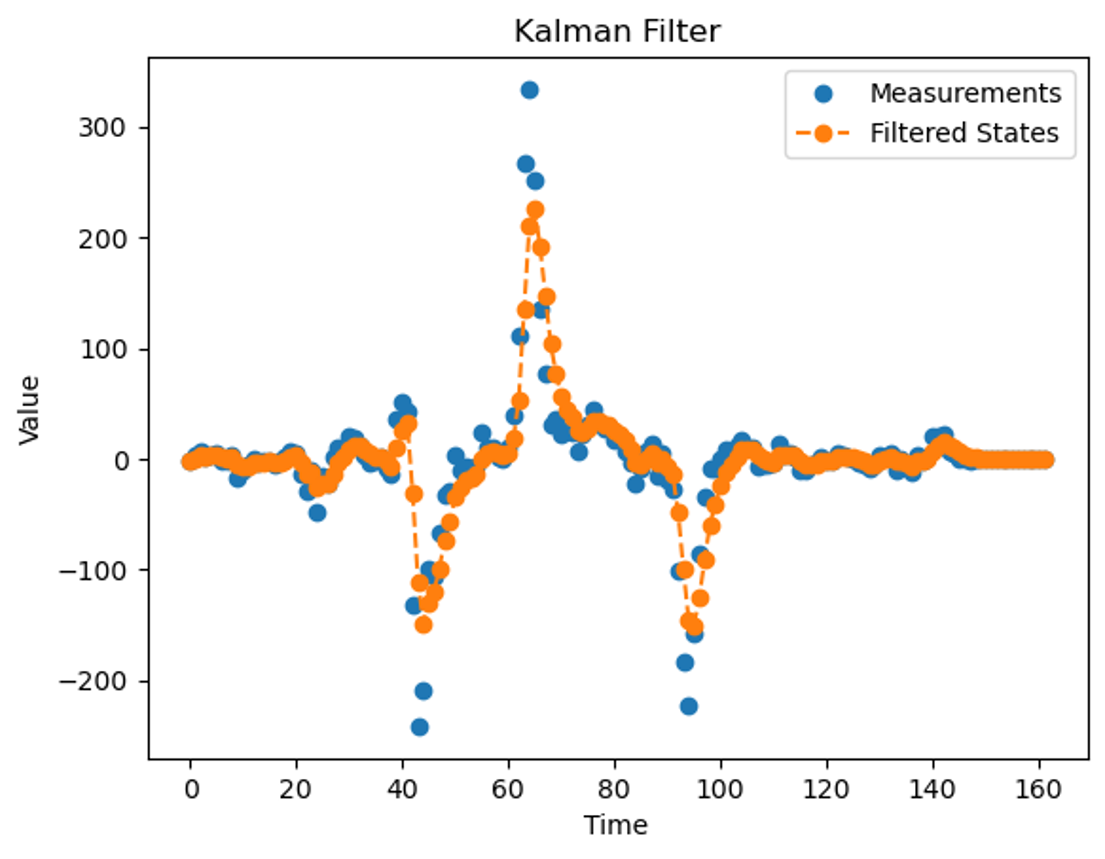
\includegraphics[scale=0.3]{Kalman}
    \caption{Kalman滤波前后数据对比(计算机上随机模拟,非压力传感器采集信号)}
    \label{Kalman}
\end{figure}
可以看到经过Kalman滤波,数据更加平滑,数据波动明显减小,对于降低噪声有作用,实验中压力传感器的显示数据波动同样得到了有效控制。
\subsection{信息传输与远程控制}
为了便于改变内腔压力和实时控制机器人生长长度,实验中将单片机与PC进行蓝牙连接,通过指令的方式对机器人实现远程控制。
\begin{figure}[H]
    \centering
    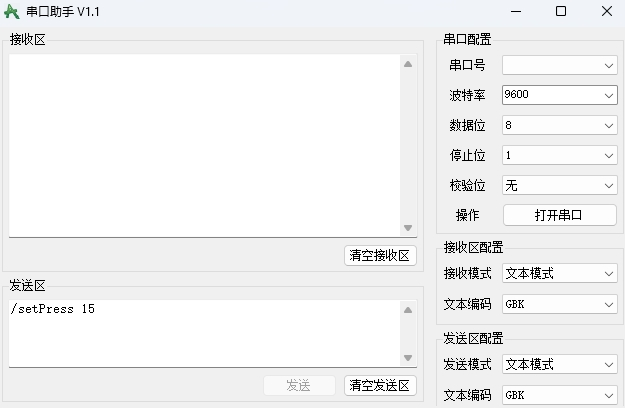
\includegraphics[scale=0.5]{操作}
    \caption{PC串口指令发送窗口}
    \label{操作}
\end{figure}

\begin{table}[H]
    \centering
    \caption{PC指令操作}
    \begin{tabular}{cc}
        \toprule
        指令格式 & 指令内容 \\ 
        \midrule
        /setPress [Value] & 将当前机器人内腔压力设置为Value kPa\\
        /to [Angle] & 将当前电机轴旋转角度设置为Angle°(含正负)\\
        \bottomrule
    \end{tabular}
\end{table}

\section{后续实验方向和要点}
1.考虑回收问题,当前暂定回收方案:分步回收,每次先排气回收一定的距离,再充气防止
薄膜堆叠,循环进行。

2.考虑转向问题方案的设计。

3.重新对基座进行设计,重点关注刚度和气密性问题,将外部元件尽可能整合到基座上,并考虑
解决塑料薄膜缠绕脱落问题的解决方案。

4.重新考虑电机和气泵的选型以适应更高气压的需要。

\section{已取得的成果}
\begin{table}[H]
    \centering
    \begin{tabular}{cc}
        \toprule
        序号 & 成果 \\ 
        \midrule
        1 & 完成了机器人激励性验证,并初步搭建实验样机\\
        2 & 完成了直线生长相关理论计算\\
        3 & 完成了电机、传感器等部件的调试,实现了机器人可控直线生长\\
        4 & 实现了机器人远程控制指令的设计和实现\\
        \bottomrule
    \end{tabular}
\end{table}

\newpage
\nocite{*}
\bibliographystyle{plain}
\bibliography{robot}

\end{document}